\appendix

\section{Training recipe}
\label{app:training}

We train on ImageNet-1k~\citep{deng2009imagenet} at $224{\times}224$.
\Cref{tab:app-training} lists the full hyper-parameter table, next to the official
ConvNeXt-T recipe~\citep{liu2022convnext}.
The four models we train from scratch share the same augmentation, regularisation and
optimiser; they differ only in peak learning rate, warmup length, minimum learning rate
and stochastic depth, as marked in the table.
The official ConvNeXt-T uses batch size $4096$ and base learning rate $4{\times}10^{-3}$.
Linear scaling to our batch of $1024$ gives $1{\times}10^{-3}$, which is the peak we use
for the weight-tied and all-stages runs.
The untied ConvNeXt-T (and its drop-path-free sibling) use half of that,
$5{\times}10^{-4}$, with the official $20$-epoch warmup.

Weight decay is applied only to convolution and linear weights (tensors of rank
$\ge 2$).
LayerNorm gain and bias, convolution/linear bias and LayerScale $\gamma$ are decay-free,
following the ConvNeXt / DeiT convention.
Convolution and linear weights are initialised with truncated normal $\mathcal{N}(0,0.02^2)$;
LayerScale uses $\gamma{=}10^{-6}$.
There is no layer-wise learning-rate decay, no gradient clipping, no mixed precision and
no exponential moving average of the weights.
The learning-rate schedule is a linear warmup (starting at $10^{-6}$) followed by cosine
decay to the listed minimum, advanced once per optimiser step.

\begin{table*}[t]
    \centering
    \caption{ImageNet-1k training settings.
    Official ConvNeXt-T from~\citet{liu2022convnext}; the remaining columns are the
    four models we train.
    CNX-T: untied baseline.
    Tied: stage~3 shares one block ($D{=}9$).
    All: one shared block per stage.
    dp0: untied ConvNeXt-T with stochastic depth off.}
    \label{tab:app-training}
    \small
    \setlength{\tabcolsep}{3.2pt}
    \begin{tabular}{lccccc}
        \toprule
        & Official & CNX-T & Tied & All & dp0 \\
        \midrule
        training epochs            & 300 & 300 & 300 & 300 & 300 \\
        warmup epochs              & 20 & 20 & 10 & 10 & 20 \\
        optimizer                  & AdamW & AdamW & AdamW & AdamW & AdamW \\
        base learning rate         & $4{\times}10^{-3}$ & $5{\times}10^{-4}$ & $1{\times}10^{-3}$ & $1{\times}10^{-3}$ & $5{\times}10^{-4}$ \\
        min.\ learning rate        & --- & $10^{-6}$ & $10^{-7}$ & $10^{-7}$ & $10^{-6}$ \\
        weight decay               & $0.05$ & $0.05$ & $0.05$ & $0.05$ & $0.05$ \\
        optimizer momentum         & $\beta{=}(0.9,0.999)$ & $\beta{=}(0.9,0.999)$ & $\beta{=}(0.9,0.999)$ & $\beta{=}(0.9,0.999)$ & $\beta{=}(0.9,0.999)$ \\
        batch size                 & $4096$ & $1024$ & $1024$ & $1024$ & $1024$ \\
        learning rate schedule     & cosine & cosine & cosine & cosine & cosine \\
        warmup schedule            & linear & linear & linear & linear & linear \\
        layer-wise lr decay        & None & None & None & None & None \\
        RandAugment                & $(9,0.5)$ & $(9,0.5)$ & $(9,0.5)$ & $(9,0.5)$ & $(9,0.5)$ \\
        Mixup $\alpha$             & $0.8$ & $0.8$ & $0.8$ & $0.8$ & $0.8$ \\
        CutMix $\alpha$            & $1.0$ & $1.0$ & $1.0$ & $1.0$ & $1.0$ \\
        random erasing             & $0.25$ & $0.25$ & $0.25$ & $0.25$ & $0.25$ \\
        color jitter               & $0.4$ & $0.4$ & $0.4$ & $0.4$ & $0.4$ \\
        label smoothing            & $0.1$ & $0.1$ & $0.1$ & $0.1$ & $0.1$ \\
        stochastic depth           & $0.1$ & $0.1$ & $0.1$ & $0.1$ & $0$ \\
        LayerScale init            & $10^{-6}$ & $10^{-6}$ & $10^{-6}$ & $10^{-6}$ & $10^{-6}$ \\
        gradient clip              & None & None & None & None & None \\
        exp.\ moving average       & None & None & None & None & None \\
        mixed precision            & --- & off & off & off & off \\
        \bottomrule
    \end{tabular}
\end{table*}

Mixup and CutMix are applied to every training batch (switch probability $0.5$), and the
loss is soft-target cross-entropy on the mixed labels.
Per-image augmentation is the timm ConvNeXt stack: random resized crop, horizontal flip,
RandAugment \texttt{rand-m9-mstd0.5}, color jitter $0.4$ and random erasing
(probability $0.25$, pixel mode).
Validation uses the standard centre crop.
Stochastic depth, when enabled, is ramped linearly from $0$ to the listed peak across the
$18$ residual blocks.

\paragraph{Stage-4 + head finetune after unrolling.}
The decoder-adaptation probe of \cref{sec:indefinite_looping} freezes stem and
stages~1--3, unrolls stage~3 at inference resolution ($R{=}100$, $\Delta t{=}0.01$,
$T{=}9$; $900$ residual steps on the weight-tied model) and trains only stage~4, the
global pool and the classification head.
We run $10$ epochs at a constant learning rate $5{\times}10^{-6}$ (no warmup, no cosine
decay), with the same optimiser, weight decay, batch size and augmentation as
\cref{tab:app-training}.

\section{Full Midpoint and RK4 refinement tables}
\label{app:solvers}

We use the same $R$ (repetitions) as in the main text: $\Delta t{=}1/R$ so that
$T{=}n$ is conserved ($n{=}9$ for ConvNeXt stage~3).
Tables~\ref{tab:app-cnx}--\ref{tab:app-r101} report plain interpolation for Euler (RK1),
Midpoint (RK2) and RK4 on each pretrained model.
\Cref{tab:app-shared-t9} gives the same solvers for the weight-tied ConvNeXt-T at
fixed horizon $T{=}9$ ($9R$ applications of the shared block).
In every case the three integrators converge to the same continuous limit once the
step is fine enough; at $R{=}1$, Mid and RK4 already sit on that limit.

\begin{table}[t]
    \centering
    \caption{ConvNeXt-T, plain, top-1 (\%).}
    \label{tab:app-cnx}
    \setlength{\tabcolsep}{4pt}
    \begin{tabular}{lrrr}
        \toprule
        $R$ & Euler & Mid & RK4 \\
        \midrule
        1   & 80.95 & 80.23 & 80.23 \\
        2   & 80.79 & 80.23 & 80.23 \\
        4   & 80.53 & 80.23 & 80.23 \\
        10  & 80.36 & 80.23 & 80.23 \\
        32  & 80.30 & 80.23 & 80.23 \\
        128 & 80.23 & 80.22 & 80.23 \\
        \bottomrule
    \end{tabular}
\end{table}

\begin{table}[t]
    \centering
    \caption{Swin-T, plain, top-1 (\%).}
    \label{tab:app-swin}
    \setlength{\tabcolsep}{4pt}
    \begin{tabular}{lrrr}
        \toprule
        $R$ & Euler & Mid & RK4 \\
        \midrule
        1   & 81.08 & 80.29 & 80.33 \\
        2   & 80.90 & 80.34 & 80.31 \\
        4   & 80.65 & 80.33 & 80.32 \\
        10  & 80.47 & 80.32 & 80.31 \\
        32  & 80.38 & 80.32 & 80.32 \\
        128 & 80.34 & 80.31 & 80.32 \\
        \bottomrule
    \end{tabular}
\end{table}

\begin{table}[t]
    \centering
    \caption{ResNet-50, plain, top-1 (\%).}
    \label{tab:app-r50}
    \setlength{\tabcolsep}{4pt}
    \begin{tabular}{lrrr}
        \toprule
        $R$ & Euler & Mid & RK4 \\
        \midrule
        1   & 80.34 & 78.94 & 79.42 \\
        2   & 80.06 & 79.41 & 79.43 \\
        4   & 79.84 & 79.44 & 79.43 \\
        10  & 79.61 & 79.44 & 79.43 \\
        32  & 79.50 & 79.43 & 79.44 \\
        128 & 79.45 & 79.43 & 79.43 \\
        \bottomrule
    \end{tabular}
\end{table}

\begin{table}[t]
    \centering
    \caption{ResNet-101, plain, top-1 (\%).}
    \label{tab:app-r101}
    \setlength{\tabcolsep}{4pt}
    \begin{tabular}{lrrr}
        \toprule
        $R$ & Euler & Mid & RK4 \\
        \midrule
        1   & 81.67 & 80.95 & 81.06 \\
        2   & 81.58 & 81.07 & 81.04 \\
        4   & 81.38 & 81.06 & 81.05 \\
        10  & 81.22 & 81.05 & 81.05 \\
        32  & 81.12 & 81.05 & 81.04 \\
        128 & 81.06 & 81.04 & 81.05 \\
        \bottomrule
    \end{tabular}
\end{table}

\begin{table}[t]
    \centering
    \caption{Shared ConvNeXt-T, fixed $T{=}9$ ($\Delta t{=}1/R$; $9R$ shared steps), top-1 (\%).}
    \label{tab:app-shared-t9}
    \setlength{\tabcolsep}{3.5pt}
    \small
    \begin{tabular}{lrrrrr}
        \toprule
        $R$ & Steps & $\Delta t$ & Euler & Mid & RK4 \\
        \midrule
        $1/9$   & 1     & 9      & 47.06 & 0.61  & 2.70 \\
        $2/9$   & 2     & 4.5    & 5.85  & 10.42 & 47.98 \\
        $3/9$   & 3     & 3      & 37.45 & 54.47 & 71.37 \\
        $4/9$   & 4     & 2.25   & 67.83 & 73.57 & 78.90 \\
        $5/9$   & 5     & 1.8    & 77.23 & 78.70 & 79.97 \\
        $6/9$   & 6     & 1.5    & 79.48 & 79.85 & 80.10 \\
        $7/9$   & 7     & 1.29   & 80.19 & 80.12 & 80.11 \\
        $8/9$   & 8     & 1.13   & 80.38 & 80.21 & 80.11 \\
        $1$     & 9     & 1      & 80.34 & 80.19 & 80.11 \\
        $4/3$   & 12    & 0.75   & 80.35 & 80.14 & 80.12 \\
        $2$     & 18    & 0.5    & 80.27 & 80.12 & 80.12 \\
        $32/9$  & 32    & 0.28   & 80.22 & 80.11 & 80.12 \\
        $128/9$ & 128   & 0.07   & 80.14 & 80.12 & 80.12 \\
        $1024/9$& 1024  & 0.009  & 80.12 & 80.12 & 80.12 \\
        $10000/9$&10000 & 0.0009 & 80.12 & ---   & --- \\
        \bottomrule
    \end{tabular}
\end{table}


\section{Solver agreement at the stage-3 endpoint}
\label{app:solver-endpoints}

\Cref{sec:indefinite_looping} asks whether a fine Euler step recovers the native
$R{=}1$ state.
A related question is whether two fine discretisations of the \emph{same} residual
field agree with each other---i.e.\ whether a continuous limit exists at all.
\Cref{tab:app-solver-endpoints} compares stage-3 endpoints $x_T$ on the same
$N{=}32$ ImageNet validation images (one per random class, seed~$0$), after zeroing
the massive channel used in the main-text metrics.
Relative distance is $\|x_a-x_b\|/\|x_b\|$; cosine is $\cos(x_a,x_b)$.

\begin{table}[t]
    \centering
    \caption{Pairwise stage-3 endpoint agreement (mean over $N{=}32$; ignore top-1
    channel). Horizon $T{=}9$ in every row.}
    \label{tab:app-solver-endpoints}
    \small
    \setlength{\tabcolsep}{3pt}
    \begin{tabular}{lrrr}
        \toprule
        Pair ($a$ vs.\ $b$) & rel.\ $\ell_2$ & $\cos$ & angle \\
        \midrule
        \multicolumn{4}{l}{\emph{ConvNeXt-T}} \\
        Euler $R{=}100$ vs.\ RK4 $R{=}100$ & $0.004$ & $1.000$ & $0.25^\circ$ \\
        Euler $R{=}100$ vs.\ Euler $R{=}200$ & $0.002$ & $1.000$ & $0.12^\circ$ \\
        Euler $R{=}100$ vs.\ Euler $R{=}1$ & $0.36$ & $0.93$ & $21^\circ$ \\
        Mid $R{=}1$ vs.\ Euler $R{=}100$ & $0.12$ & $0.993$ & $6.6^\circ$ \\
        RK4 $R{=}1$ vs.\ Euler $R{=}100$ & $0.010$ & $0.9999$ & $0.5^\circ$ \\
        \midrule
        \multicolumn{4}{l}{\emph{Weight-tied ConvNeXt-T ($9R$ shared steps)}} \\
        Euler $R{=}100$ vs.\ RK4 $R{=}100$ & $0.002$ & $1.000$ & $0.1^\circ$ \\
        Euler $R{=}100$ vs.\ Euler $R{=}200$ & $0.001$ & $1.000$ & $0.05^\circ$ \\
        Euler $R{=}100$ vs.\ Euler $R{=}1$ & $0.20$ & $0.98$ & $11^\circ$ \\
        RK4 $R{=}1$ vs.\ RK4 $R{=}100$ & $0.003$ & $1.000$ & $0.16^\circ$ \\
        \bottomrule
    \end{tabular}
\end{table}

Euler and RK4 (and Euler $R{=}100$ vs.\ $R{=}200$) collapse onto the same $x_T$, while
both remain far from the trained one-step path.
RK4 reaches that limit already with the nine unit steps of the native schedule;
the native Euler path does not.
Midpoint at $R{=}1$ matches the limit in top-1 ($80.23\%$, \cref{tab:app-cnx}) while its
state is still $12\%$ away, a reminder that accuracy is a coarse probe of $x_T$.
% TODO: optional re-run with N=500 for table error bars; script
% scripts/compare_solver_convergence.py.

\section{Random-initialisation control for the continuous limit}
\label{app:random-init}

\Cref{app:solver-endpoints} shows that the trained stage~3 has a continuous limit.
That alone is weak evidence.
Every residual field we study is a composition of Lipschitz maps (convolutions, linear
layers, normalisation, GELU/ReLU, softmax attention), so the ODE $\dot x=f_i(x)$ has a
unique solution on $[0,T]$ and Euler converges to it at first order, whatever the
weights~\citep{hairer1993solving}.
We check this empirically on all five architectures and use random fields of
controlled strength as a reference scale for the trained ones.

\paragraph{Setup.}
Every convolution and linear layer is drawn with Xavier-normal
initialisation~\citep{glorot2010understanding} (gain~$1$, zero bias, seed~$0$);
normalisation layers keep their default parameters, and ConvNeXt LayerScale is set to
$\gamma{=}1$ (its default $10^{-6}$ makes $f\approx0$).
The stage-3 blocks are then re-drawn with Xavier gain $g\in\{0.25,0.5,1,2,4,8\}$, so the
stage-3 input is identical across gains and only the field strength changes.
For ResNet the field is $f_i(x)=\mathrm{block}_i(x)-x$, which includes the ReLU applied
after the addition; for Swin one block contains both residual sub-layers (attention and
MLP), as in the main text.
For each network we integrate stage~3 to $T{=}n$ and compare the endpoint $x_T$ of Euler
at $R\in\{1,10,100,1000\}$ and of RK4 at $R{=}1$ against RK4 at $R{=}100$, on the $N{=}32$
images of \cref{app:solver-endpoints}.
The field strength is summarised by the mean relative step of the native path,
\begin{equation}
    \rho \;=\; \frac{1}{n}\sum_{i=0}^{n-1}\frac{\|f_i(x_i)\|}{\|x_i\|},
    \qquad x_{i+1}=x_i+f_i(x_i),
    \label{eq:step-ratio}
\end{equation}
i.e.\ how far a single block moves the state relative to its size.
Because $\rho$ grows with $g$ at a different rate in each architecture (about $g^3$ for
ResNet, whose bottleneck has three unnormalised convolutions), we compare trained and random networks at
matched~$\rho$: for each architecture we add one gain $g^\star$ chosen so that $\rho$
matches the trained network.
Trained ConvNeXt rows zero the massive channel (\cref{sec:massive_activations});
ResNet and Swin have no channel of comparable dominance at stage~3 (zeroing the largest
one changes every entry by less than $0.6^\circ$), so all rows except those use all
channels.

\begin{table}[t]
    \centering
    \caption{Angle between $x_T$ and the RK4 $R{=}100$ reference ($T{=}n$, mean over
    $N{=}32$). $g$: Xavier gain of the stage-3 blocks; $\rho$: mean relative step
    \eqref{eq:step-ratio}; $^\star$: gain matched to the trained $\rho$.
    Rows sorted by $\rho$.}
    \label{tab:app-random-init}
    \small
    \setlength{\tabcolsep}{3pt}
    \begin{tabular}{lrrrrr}
        \toprule
        Init & $\rho$ & \multicolumn{3}{c}{Euler} & RK4 \\
        \cmidrule(lr){3-5}
             &        & $R{=}1$ & $R{=}10$ & $R{=}100$ & $R{=}1$ \\
        \midrule
        \multicolumn{6}{l}{\emph{ConvNeXt-T (nine blocks)}} \\
        $g{=}0.5$  & 0.13 & $1.5^\circ$  & $0.15^\circ$ & $0.02^\circ$ & $0.00^\circ$ \\
        $g{=}1$    & 0.41 & $15.8^\circ$ & $1.6^\circ$  & $0.16^\circ$ & $0.07^\circ$ \\
        \textbf{Trained} & \textbf{0.54} & $\mathbf{21.1^\circ}$ & $\mathbf{2.4^\circ}$ & $\mathbf{0.25^\circ}$ & $\mathbf{0.53^\circ}$ \\
        $g^\star{=}1.35$ & 0.56 & $30.2^\circ$ & $3.4^\circ$ & $0.34^\circ$ & $0.92^\circ$ \\
        $g{=}2$    & 0.77 & $47.0^\circ$ & $6.7^\circ$  & $0.69^\circ$ & $8.4^\circ$ \\
        \midrule
        \multicolumn{6}{l}{\emph{Weight-tied ConvNeXt-T (one block)}} \\
        $g{=}0.5$  & 0.12 & $2.7^\circ$  & $0.27^\circ$ & $0.03^\circ$ & $0.00^\circ$ \\
        $g^\star{=}1$ & 0.30 & $11.9^\circ$ & $1.3^\circ$ & $0.13^\circ$ & $0.05^\circ$ \\
        \textbf{Trained} & \textbf{0.31} & $\mathbf{10.9^\circ}$ & $\mathbf{1.0^\circ}$ & $\mathbf{0.10^\circ}$ & $\mathbf{0.16^\circ}$ \\
        $g{=}2$    & 0.63 & $27.1^\circ$ & $4.3^\circ$  & $0.46^\circ$ & $5.9^\circ$ \\
        \midrule
        \multicolumn{6}{l}{\emph{ResNet-50 ($n{=}5$)}} \\
        $g{=}0.5$  & 0.04 & $0.4^\circ$  & $0.03^\circ$ & $0.00^\circ$ & $0.01^\circ$ \\
        $g{=}1$    & 0.34 & $7.0^\circ$  & $0.66^\circ$ & $0.07^\circ$ & $0.24^\circ$ \\
        $g^\star{=}1.15$ & 0.51 & $12.0^\circ$ & $1.2^\circ$ & $0.12^\circ$ & $0.48^\circ$ \\
        \textbf{Trained} & \textbf{0.52} & $\mathbf{17.0^\circ}$ & $\mathbf{1.4^\circ}$ & $\mathbf{0.15^\circ}$ & $\mathbf{0.65^\circ}$ \\
        $g{=}2$    & 2.29 & $40.6^\circ$ & $7.8^\circ$  & $0.83^\circ$ & $6.6^\circ$ \\
        \midrule
        \multicolumn{6}{l}{\emph{ResNet-101 ($n{=}22$)}} \\
        $g{=}0.5$  & 0.05 & $0.7^\circ$  & $0.05^\circ$ & $0.01^\circ$ & $0.02^\circ$ \\
        \textbf{Trained} & \textbf{0.30} & $\mathbf{15.3^\circ}$ & $\mathbf{1.4^\circ}$ & $\mathbf{0.15^\circ}$ & $\mathbf{0.74^\circ}$ \\
        $g^\star{=}0.95$ & 0.30 & $8.9^\circ$ & $0.83^\circ$ & $0.08^\circ$ & $0.29^\circ$ \\
        $g{=}1$    & 0.35 & $10.3^\circ$ & $0.97^\circ$ & $0.10^\circ$ & $0.36^\circ$ \\
        $g{=}2$    & 2.33 & $39.6^\circ$ & $5.9^\circ$  & $0.63^\circ$ & $6.4^\circ$ \\
        \midrule
        \multicolumn{6}{l}{\emph{Swin-T ($n{=}6$)}} \\
        $g{=}0.5$  & 0.15 & $1.7^\circ$  & $0.17^\circ$ & $0.02^\circ$ & $0.00^\circ$ \\
        $g{=}1$    & 0.48 & $17.2^\circ$ & $1.8^\circ$  & $0.18^\circ$ & $0.10^\circ$ \\
        \textbf{Trained} & \textbf{0.87} & $\mathbf{19.5^\circ}$ & $\mathbf{4.3^\circ}$ & $\mathbf{1.02^\circ}$ & $\mathbf{2.7^\circ}$ \\
        $g^\star{=}1.8$ & 0.89 & $47.6^\circ$ & $7.1^\circ$ & $0.74^\circ$ & $6.6^\circ$ \\
        $g{=}2$    & 0.98 & $52.7^\circ$ & $8.7^\circ$  & $0.91^\circ$ & $10.5^\circ$ \\
        \bottomrule
    \end{tabular}
\end{table}

\paragraph{Results.}
\Cref{tab:app-random-init} supports two observations.

\emph{(i)~The limit exists for every architecture.}
For every row, trained or random, the Euler error falls by roughly $10\times$ per
decade of $R$, the first-order rate (trained Swin-T is slower between $R{=}10$ and
$R{=}100$), and Euler at $R{=}1000$ is within $0.1^\circ$ of the reference.
The same holds at the larger gains not shown, with two numerical exceptions that
confirm the mechanism rather than contradict it.
ResNet at $g\ge4$ overflows in float32: without a normalisation inside the block,
$\|f_i(x)\|$ grows with $\|x\|$, so the state grows exponentially ($\rho\approx18$ per block at
$g{=}4$).
Swin at $g{=}8$ is still $15.7^\circ$ away at $R{=}1000$: the attention logits are so large
that the softmax is nearly a hard selection, the field becomes very stiff, and a finer
step is needed.
Convergence of the refinement to a single $\hat x_T$ is therefore a property of the
residual parameterisation, not something learned.

\emph{(ii)~The native gap is of the order set by $\rho$, and training moves it in an
architecture-dependent direction.}
Within each architecture the distance from the single-step path ($R{=}1$) to the limit
grows monotonically with $\rho$, and with $\rho\approx0.3$--$0.9$ every trained network
lies $10$--$21^\circ$ away: one Euler step of size~$1$ is far from tracking the flow.
At matched $\rho$, however, the trained and random networks differ, and not in a
consistent direction.
Trained Swin-T and ConvNeXt-T are \emph{closer} to their limit than a random field of the
same strength ($19.5^\circ$ vs.\ $47.6^\circ$ and $21.1^\circ$ vs.\ $30.2^\circ$), the
weight-tied model is level with it ($10.9^\circ$ vs.\ $11.9^\circ$), and both ResNets are
\emph{farther} ($17.0^\circ$ vs.\ $12.0^\circ$ and $15.3^\circ$ vs.\ $8.9^\circ$).
RK4 at $\Delta t{=}1$ follows the same split.
Training thus changes how well a single step approximates the flow, but there is no
universal tendency for single-use blocks to be better (or worse) one-step solvers than
random ones.
Script: \texttt{scripts/random\_init\_convergence.py}.
% Raw numbers: outputs/random_init_convergence/xavier.csv

\section{Block permutation, duplication and substitution}
\label{app:block-ops}

% TODO: report ImageNet val ablations on pretrained ConvNeXt stage~3
% (permute block order, duplicate / drop blocks, replace all blocks by a middle one),
% in the spirit of \citet{sun2025painters}.

\section{Bilinear weight interpolation}
\label{app:bilinear}

Continuous-in-depth work often assumes a smooth path in weight space between consecutive
blocks~\citep{queiruga2020continuousindepthneuralnetworks,chang2018multilevel},
\begin{equation}
    \theta(t) \;=\; (1-\alpha)\,\theta_i + \alpha\,\theta_{i+1},
    \qquad \alpha = t - i.
    \label{eq:bilinear-theta}
\end{equation}
Replacing the plain schedule $\theta_t=\theta_{\lfloor t\rfloor}$ by~\eqref{eq:bilinear-theta}
hurts every model we tested: at $R{=}128$ the drop vs.\ plain is between $6.6$ and $23.3$
points (\cref{tab:app-bilinear}).
Consecutive blocks are not neuron-aligned, so the midpoint of their weights is not a
functional intermediate~\citep{entezari2022permutation,ainsworth2023gitrebasin}.

\begin{table}[t]
    \centering
    \caption{Bilinear weight interpolation, Euler, top-1 (\%).}
    \label{tab:app-bilinear}
    \small
    \setlength{\tabcolsep}{2.8pt}
    \begin{tabular}{lrrrrr}
        \toprule
        $R$ & CNX-T & CNX-T$^{\dagger}$ & Swin-T & R-50 & R-101 \\
        \midrule
        1   & 80.96 & 79.27 & 81.08 & 80.34 & 81.67 \\
        2   & 78.94 & 72.43 & 78.93 & 74.95 & 72.55 \\
        4   & 76.16 & 63.13 & 75.42 & 70.60 & 62.42 \\
        10  & 74.42 & 58.75 & 73.28 & 68.58 & 58.73 \\
        128 & 73.66 & 57.44 & 72.14 & 67.77 & 57.73 \\
        \midrule
        $\Delta$ vs plain @128 & $-6.6$ & $-19.6$ & $-8.2$ & $-11.7$ & $-23.3$ \\
        \bottomrule
    \end{tabular}
    \vspace{2pt}
    {\footnotesize $^{\dagger}$ConvNeXt-T trained without drop path.}
\end{table}

\Cref{fig:bilinear-norm} shows the ConvNeXt residual-field norm under plain vs.\ bilinear
schedules at $R{=}100$.
Plain keeps the piecewise-constant staircase of \cref{fig:refinement}~(right);
bilinear adds high-frequency oscillation between block boundaries while preserving the
same global growth of $\|f\|$.
Bands are P5--P95 across 500 validation images (same suite as \cref{fig:refinement}).

\begin{figure}[t]
    \centering
    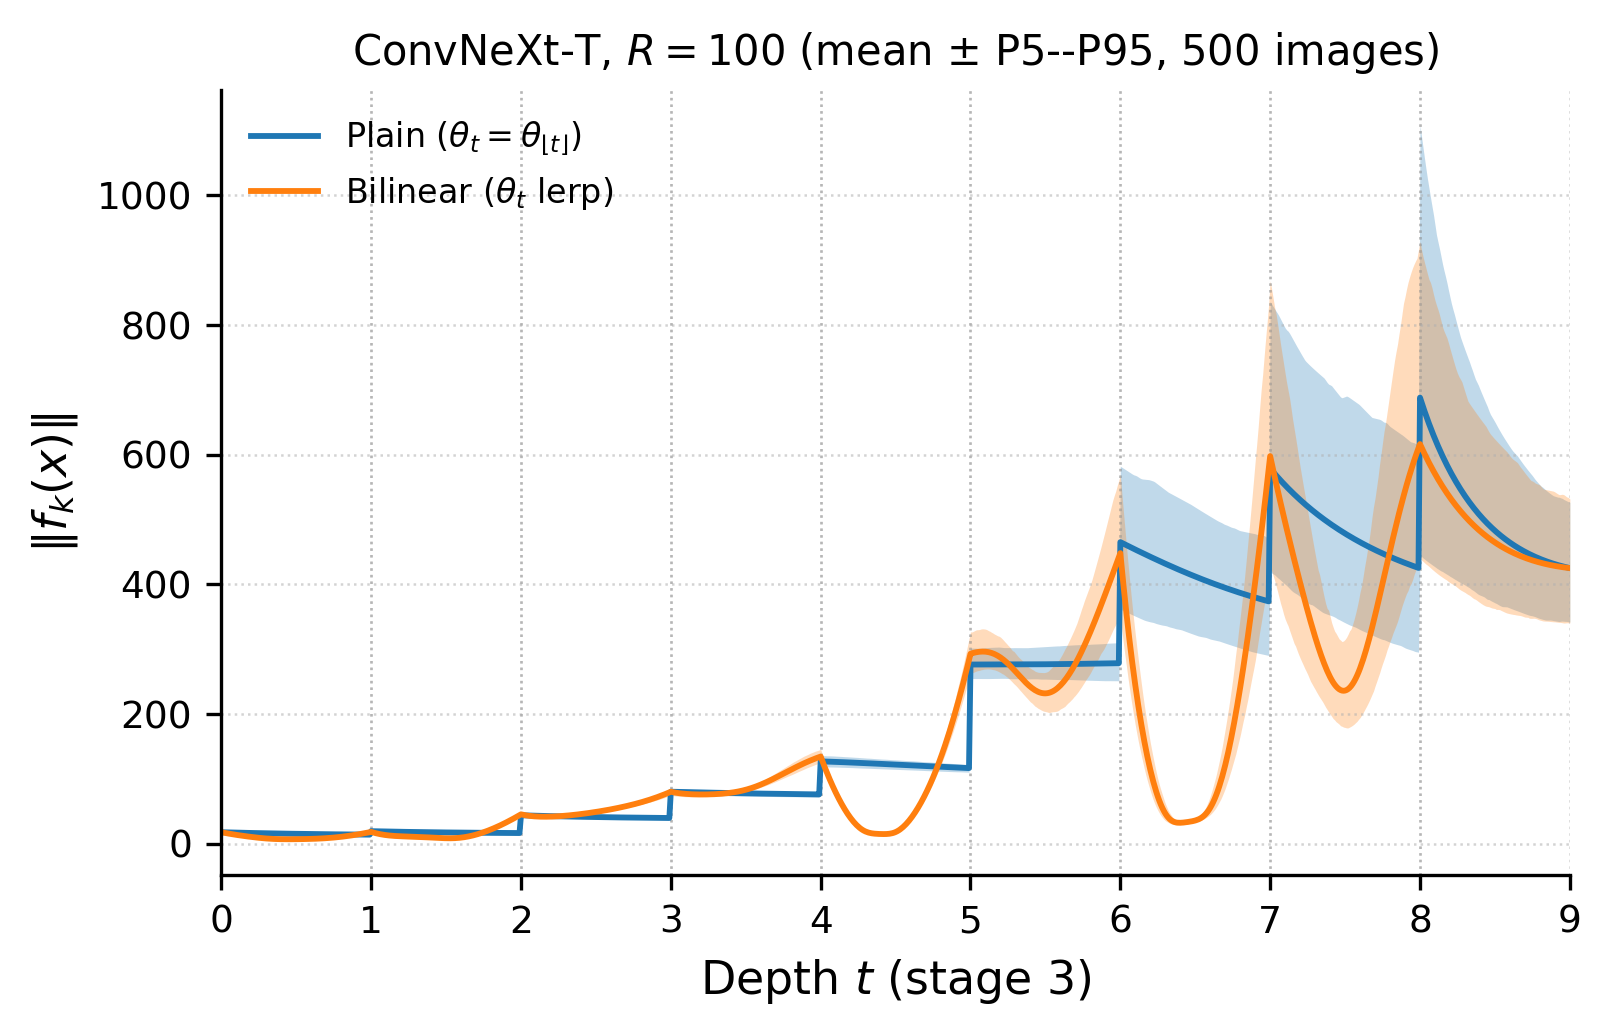
\includegraphics[width=\linewidth]{figures/bilinear_norm.png}
    \caption{ConvNeXt-T residual norm along stage~3 at $R{=}100$:
    plain vs.\ bilinear weight interpolation (mean and P5--P95 over 500 images).}
    \label{fig:bilinear-norm}
\end{figure}
